\documentclass [aspectratio=169]{beamer}
\usetheme{Boadilla}
\usepackage{textpos} % package for the positioning
\usepackage[]{graphicx}
\usepackage{graphicx}
\usepackage{float}
\usepackage{hyperref}
\usepackage{caption}
\usepackage{subcaption}
\usepackage{algorithm,algpseudocode}
\usepackage[export]{adjustbox}
\usepackage{tikz}
\usetikzlibrary{positioning}
\usetikzlibrary{arrows, shapes, decorations, automata, backgrounds, fit, petri, calc}

\definecolor{uoftblue}{RGB}{6,41,88} % official blue color for uoft


\title[]{Development of digital twin via generative neural networks}
%\subtitle{Using Beamer}
\author[]{Kuilin Chen}
%\institute[]{University of Toronto}
\date{\today}

% set color
\setbeamercolor{title in head/foot}{bg=white}
\setbeamercolor{author in head/foot}{bg=white}
\setbeamercolor{date in head/foot}{fg=uoftblue}
\setbeamercolor{date in head/foot}{bg=white}
\setbeamercolor{title}{fg=uoftblue}
\setbeamercolor{frametitle}{fg=uoftblue}

% set logo at non-title pages
\logo{
\includegraphics[height=0.8cm]{logo_uoft.png}\vspace*{-.055\paperheight}\hspace*{.85\paperwidth}}

\begin{document}

{
\setbeamertemplate{logo}{}
\begin{frame}
    \titlepage
    \begin{textblock*}{4cm}(0.5cm,-7cm)
        
\includegraphics[width=4cm]{logo_uoft.png}
    \end{textblock*}
    \begin{textblock*}{4cm}(4.8cm,-6.3cm)
        \huge \color{uoftblue}{$\vert$ Engineering}
    \end{textblock*}
\end{frame}
}

\begin{frame}{Outline}
    \begin{itemize}
    	\item Review of previous work
        \item Review of generative neural network
        \item Dynamic generative neural network
        \item Seq2Seq generation
        \item Future work
    \end{itemize}
    
\end{frame}

\begin{frame}{Previous work}
    \begin{itemize}
        \item Completed the literature review of digital twin and pointed out research opportunities in current digital twin research
        \item Current research focus is to model the relationship between set points and actual temperature inside combustion system
        \item ARX, LSTM and GRU models have been developed to predict one-step-ahead temperature based on past set points and temperature 
        \item Try to develop new generative models for time-series 
    \end{itemize}
\end{frame}



\begin{frame}{Generative neural network}
    \begin{itemize}
        \item We want to learn a probability distribution over high-dimensional $x$ (e.g. picture and long time-series)
        \item $p_{\mathcal{D}}(x)$ is the true distribution, and $p_{\theta}(x)$ is the modelled distribution
        \item Direct optimization over $p_{\theta}$ to approximate $p_{\mathcal{D}}$ is very challenging (e.g. high-dimensionality, existence of $p_{\mathcal{D}}$...)
        \item We define a low-dimensional $z$ with a fixed prior distribution $p(z)$, and pass $z$ through $g_{\theta}$ (deep neural network): $\mathcal{Z} \rightarrow \mathcal{X}$
        \item High-dimensional $x$ can be generated without explicitly knowing high-dimensional density
    \end{itemize}
\end{frame}

\begin{frame}{Generative adversarial networks (GAN)}
    \begin{block}{Adversarial training}
        \begin{equation*}
            \min _{G} \max _{D} V(D, G)=\mathbb{E}_{{x} \sim p_{\mathcal { D }}({x})}[\log D({x})]+\mathbb{E}_{{z} \sim p_{{z}}}({z})[\log (1-D(G({z})))]
        \end{equation*}
    \end{block}
    \begin{itemize}
        \item $G$ is a generator, $D$ is a discriminator
        \item Train $D$ to discriminate the real and generated samples
        \item Simultaneously train $G$ to generate samples close to real samples
        \item $p(x)$ is not explicitly modeled in GAN
        \item Evaluation of generated samples from GAN can be done by human subjectively
    \end{itemize}
\end{frame}


\begin{frame}{Variational autoencoder (VAE)}
    \begin{block}{Evidence lower bound (ELBO)}
        \begin{equation*}
            \mathcal{L}(x)=\underbrace{\color{blue}-D_{\mathrm{KL}}\left(q_{\phi}(z | x) \| p(z)\right) }_{\text{regularization}}+ \underbrace{\color{red}\mathbb{E}_{q_{\phi}(z | x)}\left[\log p_{\theta}(x | z)\right]}_{\text{log-likelihood}}
        \end{equation*}
	\end{block}
	\begin{itemize}
        \item $q_{\phi}(z | x)$ is a probabilistic encoder, $p_{\theta}(x | z)$ is a probabilistic decoder
        \item Maximize $\mathcal{L}$ by varying $\phi$ and $\theta$ to train the generative model
        \item ELBO or log-likelihood could be maximized by overfitting $x$ (memorize the training sample)
        \item Good ELBO or log-likelihood values does not imply good inference
        \item ELBO or log-likelihood should not be used to evaluate generated samples
    \end{itemize}
\end{frame}


\begin{frame}{RNN and SSM}

    \begin{figure}[H]%
        \centering%
        \begin{subfigure}{.48\textwidth}%
          \centering
          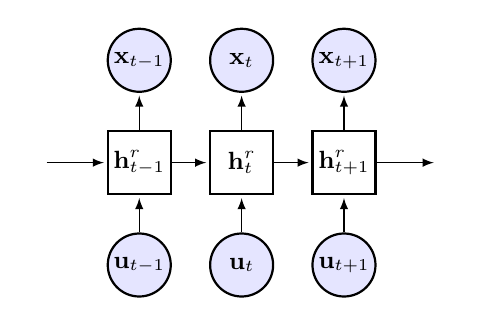
\begin{tikzpicture}[bend angle=45,>=latex, font=\small,scale=1, every node/.style={transform shape}]%
        
            \tikzstyle{obs} = [ circle, thick, draw = black!100, fill = blue!10, minimum size = 0.8cm, inner sep = 0pt]
            \tikzstyle{lat} = [ circle, thick, draw = black!100, fill = red!0, minimum size =  0.8cm, inner sep = 0pt]
            \tikzstyle{par} = [ circle, thin, draw, fill = black!100, minimum size = 0.8, inner sep = 0pt]	
            \tikzstyle{det} = [ rectangle, thick, draw = black!100, fill = red!0, minimum size = 0.8cm, inner sep = 0pt]
            \tikzstyle{inv} = [ circle, thin, draw=white!100, fill = white!100, minimum size = 0.8cm, inner sep = 0pt]	
            \tikzstyle{every label} = [black!100]%
        %%
            \begin{scope}[node distance = 1.3cm and 1.3cm]%
                %% State variables
                \node (hr_tm2) {};
                \node [det] (hr_tm1) [ right of = hr_tm2]   {$\mathbf{h}_{t-1}^r$};
                \node [det] (hr_t) [ right of = hr_tm1]   {$\mathbf{h}_{t}^r$};
                \node [det] (hr_tp1) [ right of = hr_t] {$\mathbf{h}_{t+1}^r$};
                \node (hr_tp2) [ right of = hr_tp1]{};
                
                
            
                \draw[post] (hr_tm2) edge  (hr_tm1);
                \draw[post] (hr_tm1) edge  (hr_t);
                \draw[post] (hr_t) edge  (hr_tp1);
                \draw[post] (hr_tp1) edge  (hr_tp2);
                
                
                %% Outputs
                \node [obs] (x_tm1) [ above of = hr_tm1]   {$\mathbf{x}_{t-1}$};
                \node [obs] (x_t) [ above of = hr_t] {$\mathbf{x}_{t}$};
                \node [obs] (x_tp1) [ above of = hr_tp1] {$\mathbf{x}_{t+1}$};
                
                \draw[post] (hr_tm1) edge  (x_tm1);
                \draw[post] (hr_t) edge  (x_t);
                \draw[post] (hr_tp1) edge (x_tp1);
                
                %% Inputs
                \node [obs] (u_tm1) [ below of = hr_tm1]   {$\mathbf{u}_{t-1}$};
                \node [obs] (u_t) [ below of = hr_t] {$\mathbf{u}_{t}$};
                \node [obs] (u_tp1) [ below of = hr_tp1] {$\mathbf{u}_{t+1}$};
                
                \draw[post] (u_tm1) edge  (hr_tm1);
                \draw[post] (u_t) edge  (hr_t);
                \draw[post] (u_tp1) edge  (hr_tp1);	
                
                
            \end{scope}%
        \end{tikzpicture}%
          \caption{RNN}%
          \label{fig:rnn}%
        \end{subfigure}%
        \begin{subfigure}{.48\textwidth}%
          \centering%
          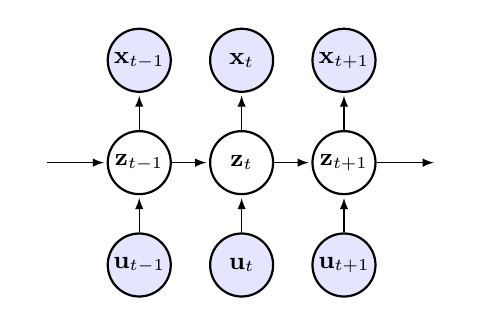
\begin{tikzpicture}[bend angle=45,>=latex, font=\small,scale=1, every node/.style={transform shape}]%
        
            \tikzstyle{obs} = [ circle, thick, draw = black!100, fill = blue!10, minimum size = 0.8cm, inner sep = 0pt]
            \tikzstyle{lat} = [ circle, thick, draw = black!100, fill = red!0, minimum size =  0.8cm, inner sep = 0pt]
            \tikzstyle{par} = [ circle, thin, draw, fill = black!100, minimum size = 0.8, inner sep = 0pt]	
            \tikzstyle{det} = [ diamond, thick, draw = black!100, fill = red!0, minimum size = 1cm, inner sep = 0pt]
            \tikzstyle{inv} = [ circle, thin, draw=white!100, fill = white!100, minimum size = 0.8cm, inner sep = 0pt]	
            \tikzstyle{every label} = [black!100]%
        %
            \begin{scope}[node distance = 1.3cm and 1.5cm]
                %% State variables
                \node (h_tm2) {};
                \node [lat] (h_tm1) [ right of = h_tm2]   {$\mathbf{z}_{t-1}$};
                \node [lat] (h_t) [ right of = h_tm1]   {$\mathbf{z}_{t}$};
                \node [lat] (h_tp1) [ right of = h_t] {$\mathbf{z}_{t+1}$};
                \node (h_tp2) [ right of = h_tp1]{};
                
            
                \draw[post] (h_tm2) edge  (h_tm1);
                \draw[post] (h_tm1) edge  (h_t);
                \draw[post] (h_t) edge  (h_tp1);
                \draw[post] (h_tp1) edge  (h_tp2);
        
                
                %% Outputs
                \node [obs] (x_tm1) [ above of = h_tm1]   {$\mathbf{x}_{t-1}$};
                \node [obs] (x_t) [ above of = h_t] {$\mathbf{x}_{t}$};
                \node [obs] (x_tp1) [ above of = h_tp1] {$\mathbf{x}_{t+1}$};
                
                \draw[post] (h_tm1) edge  (x_tm1);
                \draw[post] (h_t) edge  (x_t);
                \draw[post] (h_tp1) edge  (x_tp1);
        
                %% Inputs
                \node [obs] (u_tm1) [ below of = h_tm1]   {$\mathbf{u}_{t-1}$};
                \node [obs] (u_t) [ below of = h_t] {$\mathbf{u}_{t}$};
                \node [obs] (u_tp1) [ below of = h_tp1] {$\mathbf{u}_{t+1}$};
                
                \draw[post] (u_tm1) edge  (h_tm1);
                \draw[post] (u_t) edge  (h_t);
                \draw[post] (u_tp1) edge  (h_tp1);	
        
            \end{scope}
        \end{tikzpicture}%
          \caption{SSM}%
          \label{fig:ssm}%
        \end{subfigure}%
        \caption{Graphical models to generate $\mathbf{x}_{1:T}$ with a recurrent neural network (RNN) and a state space model (SSM).
        Rectangle-shaped units are used for deterministic states, while circles are used for stochastic ones.
        }%
        \label{fig:test}%
    \end{figure}%
    
    \begin{columns}
		\begin{column}{0.5\textwidth}
   		\begin{equation*}
   			\begin{array}{l}{\mathbf{h}_{t}=f\left(\mathbf{h}_{t-1}, \mathbf{u}_{t}\right)} \\ {\mathbf{x}_{t}=g\left(\mathbf{h}_{t}\right)}\end{array}
   		\end{equation*}
		\end{column}
		\begin{column}{0.5\textwidth}
			\begin{equation*}
				\begin{array}{l}{\mathbf{z}_{t} \sim p_{\theta_{z}}\left(\mathbf{z}_{t} | \mathbf{u}_{t}, \mathbf{z}_{t-1}\right)} \\ {\mathbf{x}_{t} \sim p_{\theta_{x}}\left(\mathbf{x}_{t} | \mathbf{z}_{t}\right)}\end{array}
			\end{equation*}
		\end{column}
\end{columns}

\end{frame}


\begin{frame}{Combination of RNN and SSM}
    \begin{itemize}
    	\item RNN and SSM have been combined to develop generative models in some papers
    	\item However, their models are limited to categorical input and output (e.g. rotated image generate, new drug development)
    	\item A new generative model is proposed based on combination of bi-directional RNN and SSM
    	\item The objective function and output decoding distribution are re-designed to make it suitable for time-series generation
    \end{itemize}
\end{frame}



\begin{frame}{Variational inference for dynamic generative model}
	\begin{block}{ELBO}
	\begin{equation*}
		\begin{aligned} 
		& \log p_{\theta}(\mathbf{x} | \mathbf{u})-\mathcal{D}_{K L}\left(q_{\phi}(\mathbf{z} | \mathbf{x}, \mathbf{u}) \| p_{\theta}(\mathbf{z} | \mathbf{x}, \mathbf{u})\right) \\
		=& \underbrace{\color{red}\mathbb{E}_{\mathbf{z} \sim q_{\phi}}\left[\log p_{\theta}(\mathbf{x} | \mathbf{z}, \mathbf{u})\right]}_{\text{log-likelihood}}-\underbrace{\color{blue}\mathcal{D}_{K L}\left[q_{\phi}(\mathbf{z} | \mathbf{x}, \mathbf{u}) \| p_{\theta}(\mathbf{z} | \mathbf{u})\right]}_{\text{regularization}} \\
		=& \mathcal{L}(\theta, \phi) \end{aligned}
	\end{equation*}	
	\end{block}
	


\end{frame}

\begin{frame}{Algorithm}

    \begin{algorithm}[H]
        \caption{Dynamic generative model}
        \begin{algorithmic}
        \State Initialize parameters $\theta, \phi$ 
        \Repeat
        \State Get random minibatch datapoints $\mathbf{x}, \mathbf{u}$
        \State Get Monte Carlo samples $\mathbf{z}^* $ from distribution $q_{\phi}(\mathbf{z}|\mathbf{x}, \mathbf{u})$
        \State Evaluate $\mathbb{E}_{\mathbf{z} \sim q_{\phi}} [\log p_{\theta}(\mathbf{x}|\mathbf{z}, \mathbf{u})]$ using $\mathbf{z}^* $
        \State Update parameters using gradients $\nabla_{\theta,\phi}\mathcal{L}$ (e.g. SGD)
        \Until {convergence of parameters $\theta,\phi$}
        \\ \Return $\theta, \phi$
        \end{algorithmic}
        \label{algorithm}
    \end{algorithm}
	
\end{frame}

\begin{frame}
    \begin{center}
        \Huge Thank You!\\
        \Huge Questions?
    \end{center}
\end{frame}


\end{document}
